%%%%%%%%%%%%%%%%%Epic 12%%%%%%%%%%%%%%%%%%%%%%%%%%%%%%%%%%%%%%%%%%%%%%%%%%%%%%%
\subsection{Ziel erreichen}

Es ist das gefordert, dass der Roboter sicher weiss, dass er sich im Ziel befindet und dies erkenntlich gibt mit einem Buzzer Geräusch, welches schon im vorangegangenen Kapitel \ref{peripherie-buzzer} beschriebene ist.

\subsubsection{Zielknoten erkennen}
\label{detect-target}

Es wurde bereits in \acrshort{pren1} die Methode gewählt, mit welcher die Buchstaben auf den Zielknoten erkannt werden sollen. Dieser Code muss nun lediglich migriert werden, um in die Architektur der Navigation zu passen.

Wie geplant wird der \gls{orb-gloss} Algorithmus verwendet, der in der OpenCV Library vorhanden ist. Es wird die TargetNodeReader Klasse im NodeReader Modul erstellt (siehe Grafik \ref{fig:nav-arch}). Sobald eine Instanz dieser Klasse erstellt wird, lernt sie die Konturen von den Buchstaben A, B und C und speichert diese in Attributen.
Dies lernt sie von Beispielbildern von den schwarzen Buchstaben auf weissem Hintergrund.
Jedes Mal, wenn der Roboter einen Knoten fotografiert, wird dieses Bild verzerrt, um den Knoten in Vogelperspektive anzuzeigen (siehe Kapitel \ref{outgoing-lines}) und dann wird detektiert, ob sich darauf der Buchstabe des Zielknotens befindet. Falls der Zielknoten sich darauf befindet, macht der Roboter ein Buzzergeraeusch (siehe Kapitel \ref{peripherie-buzzer}).

Auf folgender Grafik ist die Klasse in Verhältnis zu dem Navigator dargestellt.

\begin{figure}[H]
\centering
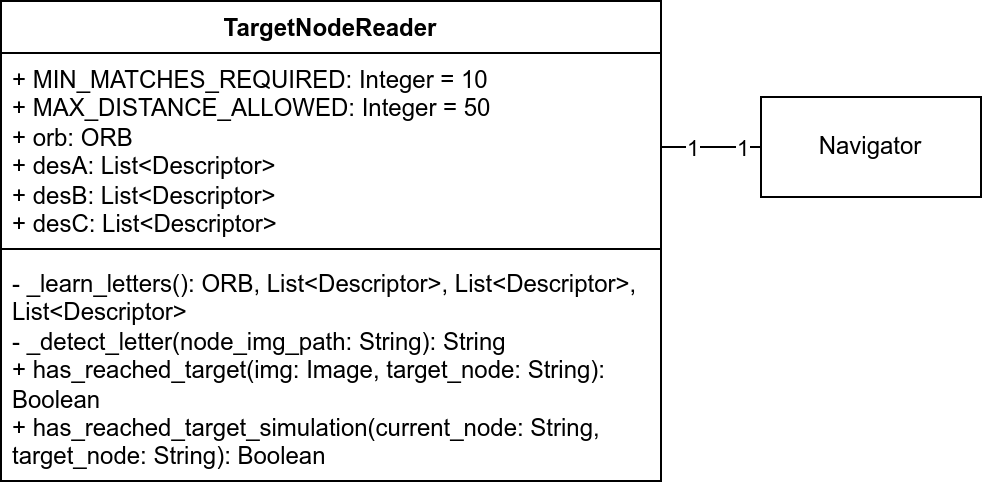
\includegraphics[width=\textwidth]{assets/IT/robot-sw-architecture-target-node-detector.png}
\caption{TargetNodeDetector Klassendiagramm}
\label{fig:target-node-nav}
\end{figure}

\acrshort{orb} gibt jeweils zurück, wie nahe die Anhaltspunkte des richtigen Objektes den Beispielbildern, die er gelernt hat, ist. Damit die Navigation in der Lage ist sowohl den richtigen Buchstaben zu erkennen, als auch jegliche Absenz eines Buchstabens, muss definiert werden, wie sicher der Algorithmus sich sein muss, dass es sich um einen Buchstaben handelt, damit es akzeptiert wird. Dafür wurden die folgenden zwei Parameter definiert:
\begin{verbatim}
# Anzahl Anhaltspunkte die gefunden werden müssen
MIN_MATCHES_REQUIRED = 10
# Wie unterschiedlich die Anhaltspunkte sein dürfen,
# um immer noch als Match zu zählen
MAX_DISTANCE_ALLOWED = 50
\end{verbatim}

Eine genaue Erklärung dieser Parameter, sowie ein Protokoll, wie die Werte ermittelt wurden koennen im Anhang im Kapitel \nameref{target-node-unittests} gefunden werden.

Diese Funktionalität wurde erneut mit Unittests getestet.
Dabei wird die Klasse, die die Konturen der Buchstaben lernt instanziert und dann werden realistische Bilder an die Methode übergeben, die die Knoten liest. Alle Buchstaben inklusive Knoten ohne Buchstaben werden richtig erkannt. Diese Tests sind ebenfalls im Anhang im Kapitel \nameref{target-node-unittests} zu finden.

Durch die ausführlichen Tests kann das Risiko 22, dass der Roboter das Ziel verpasst oder es sich eingebildet, sehr stark mitigiert werden.

Damit die Navigation nach wie vor auf allen Umgebungen laufen kann, werden hier zwei Methoden erstellt, eine Dummy Methode, die aus dem Simulator übernommen wurde und die richtige Methode, die Buchstaben von Bildern detektiert. so kann einfach hin und her gewechselt werden je nach Umgebung.


\newpage
%%%%%%%%%%%%%%%%%Epic 13%%%%%%%%%%%%%%%%%%%%%%%%%%%%%%%%%%%%%%%%%%%%%%%%%%%%%%%
\subsection{Funktion-Stop}


Der Hauptschalter ist leicht zugänglich vorn am Roboter angebracht und trennt alle  relevanten Funktionen zuverlässig vom Stromkreis. Befindet sich der Schalter in der unteren Stellung, ist das Fahrzeug vollständig deaktiviert.

Eine Ausnahme bildet der Raspberry Pi, der auch bei deaktiviertem Hauptschalter weiterhin mit Strom versorgt wird. Dies ist bewusst so vorgesehen, um Datenverlust oder Dateisystemfehler durch unerwartetes Abschalten zu vermeiden.
...... POSSIBLY Bild von Verkablungsschema

\subsubsection{Schaltergehäuse}

Am Schaltergehäuse werden der Hauptschalter und die zwei Inputtasten für die Zielauswahl und das Startsignal montiert. Das Gehäuse steht leicht erhöht auf Grundplatte. Unter dem Gehäuse werden die Kabel für den Ultraschallsensor durchgeführt.



\begin{figure}[H]
\centering
\includegraphics[width=0.5\textwidth, angle=-90]{assets/MT/Schaltergehäuse.jpg}
\caption{Schaltergehäuse}
\label{fig:Schaltergehäuse}
\end{figure}

